\chapter{Формирование требований к системе}

\section{Анализ предметной области}

Разрабатываемая в компании Cera Marketing система позволяет находить маршруты людей, моменты входа и выхода людей в определенные зоны, а также определять моменты контакта разных людей в определенных зонах. При этом, в отличии от аналогов, система способна работать с видео, снятом с обычных камер видеонаблюдения с практически любых углов. В связи с этим возникает необходимость предварительно настраивать алгоритм для каждого конкретного случая.

% Типичный процесс обработки видео состоит из нескольких этапов:

% \begin{enumerate}
%   \item подбор оптимальных параметров для алгоритма;
%   \item разметка изображения с камеры на зоны;
%   \item запуск алгоритма;
%   \item визуальная проверка качества работы алгоритма.
% \end{enumerate}


\subsection{Актуальность разработки}

Алгоритмы компьютерного зрения очень требовательные с точки зрения потребления ресурсов компьютера. Обработка 3-х часового видео на современном компьютере занимает по времени около 10 минут — это значит, что обрабатывать видео больше чем с 18 камер в день на сервере с одним процессорным ядром невозоможно. В связи с этим встает вопрос о параллельной обработке данных на нескольких компьютерах.

Для сокращения издержек и упрощения процессов поддержки физических серверов, актуально использование услуг провайдеров облачных решений. Многие компании предоставляют вычислительные мощности <<по требованию>>. Такие мощности обходятся гораздо дешевле, чем поддержка собственного дата-центра.

Однако, некоторые крупные клиенты очень скептически относятся к идее передачи данных другой компании. Им хотелось бы лицензировать ПО и использовать его самостоятельно, на собственных серверах. Таким образом, еще одной важной деталью является возможность автоматизации развертки ПО не только в облаке, но и впринципе на любых компьютерах.

\begin{figure}
  \centering
  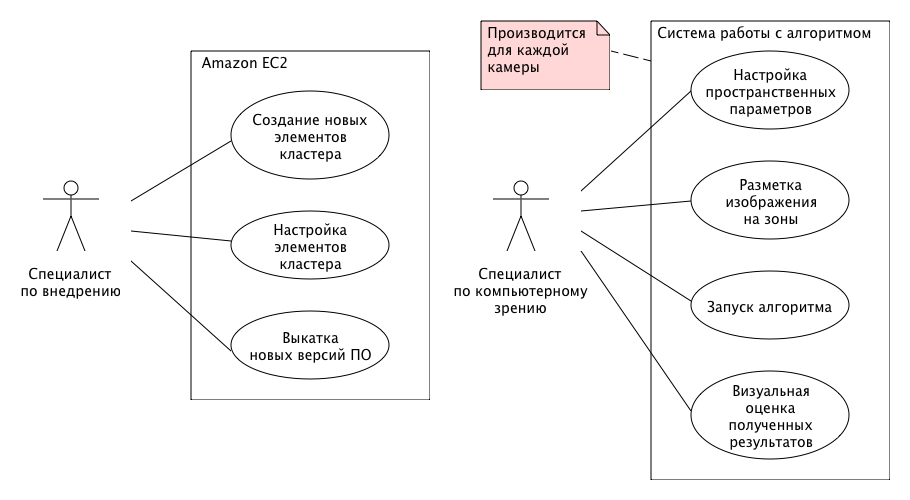
\includegraphics[width=0.8\textwidth]{assets/use-case-1.png}
  \caption{Диаграмма вариантов использования}
  \label{fig:fig01}
\end{figure}

Ко всему прочему, для каждой новой камеры параметры алгоритма необходимо подстраивать, изображение размечать на зоны, а также периодически визуально проверять качество работы. Если речь идет о нескольких видео, все это можно делать при помощи подручных средств на своем компьютере, однако если нужно работать с несколькими камерами в день встает вопрос об автоматизации процесса и передачи его в руки неподготовленного персонала.

\section{Обзор и анализ аналогов}

Прямых аналогов разрабатываемой системе не обнаружено, так как задача является очень специфической. Однако, в качестве аналогов можно рассмотривать более общие системы управления вычислительными кластерами.

\subsection{MOSIX2}
MOSIX2 — это система управления кластерами и сетями ОС на ядре Linux, представляющая их как одну систему (Single-System Image, SSI), то есть эквивалент операционной системы для кластера в целом. В кластере MOSIX2 нет необходимости в модификации существующих приложений, в связывании с дополнительными библиотеками, в явном входе на удаленные узлы — все это осуществляется автоматически на уровне ОС.

Пользователи запускают свои обычные приложения (как последовательные так и параллельные) и MOSIX прозрачно для них ищет свободные ресурсы в кластере и распределяет процессы среди доступных узлов, увеличивая тем самым общую производительность.

\subsection{MPI / Open MPI}
Программный интерфейс (API) для передачи информации, который позволяет обмениваться сообщениями между процессами. Разработан Уильямом Гроуппом, Эвином Ласком (англ.) и другими.

Базовым механизмом связи между MPI процессами является передача и приём сообщений. Сообщение несёт в себе передаваемые данные и информацию, позволяющую принимающей стороне осуществлять их выборочный приём:
\begin{enumerate}
  \item отправитель — ранг (номер в группе) отправителя сообщения;
  \item получатель — ранг получателя;
  \item признак — может использоваться для разделения различных видов сообщений;
  \item коммуникатор — код группы процессов.
\end{enumerate}
Операции приёма и передачи могут быть блокирующимися и не блокирующимися. Для не блокирующихся операций определены функции проверки готовности и ожидания выполнения операции.





% будут рассмотрены две категории аналогов — решения для анализа статистики :
% \subsection{Синезис Кассиопея}
% Видеоаналитическое решение по сбору статистики и анализу данных для бизнеса, ритейла, транспорта, общественных организаций. Бизнес-аналитика автоматически обрабатывает видеопоток с камер, анализирует видео по заданным правилам, собирает статистику и передает ее на центральный сервер.

\section{Формирование требований}

До разработки всей системы в компании Cera Marketing было произведено большое исследование потребностей клиентов, а так же исследование конкурентов.
Основными источниками требований послужили:
\begin{enumerate}
  \item представления и ожидания клиентов компании;
  \item конкурирующие программные продукты;
  % \item представления и ожидания пользователей системы;
  \item текущая организация деятельности в организации.
\end{enumerate}

\subsection{Требования к системе}

Основные требования к системе развертки:

\begin{enumerate}
  \item Возможность полной автоматической настройка ОС компьютеров кластера, а именно:
  \begin{enumerate}
    \item создание новых пользователей
    \item установка всех необходимых зависимостей
    \item установка нашего ПО
    \item базовая настройка всех компонентов ПО и зависимостей
  \end{enumerate}
  \item Автоматизация развертывание новых версий ПО:
  \begin{enumerate}
    \item обновление ПО
    \item настройка всех компонентов
    \item миграция базы данных
    \item установка новых зависимостей
  \end{enumerate}
  \item Управление элементами кластера в системе Amazon EC2, а именно:
  \begin{enumerate}
    \item запуск, остановка элементов кластера
    \item создание, удаление элементов кластера
    \item клонирование элементов кластера
  \end{enumerate}
\end{enumerate}

Требования к системе управления кластером:
\begin{enumerate}
  \item Возможность настройки пространственных параметров алгоритма
  \item Разметка картинки с камеры на зоны
  \item Запуск обработки видео
  \item Визуальная оценка качества полученных результатов
\end{enumerate}

\subsection{Требования к ПО пользователей}
Система должна работать на компьютерах под управлением всех из нижеперечисленных ОС:
\begin{enumerate}
  \item Любая ОС на базе Linux;
  \item Windows XP или выше;
  \item Mac OS X.
\end{enumerate}

и всех из нижеперечисленных браузеров:
\begin{enumerate}
  \item Google Chrome версии 6.0 или выше;
  \item Mozilla Firefox версии 4.0 или выше;
\end{enumerate}

Система развертки может быть более требовательна к ПО, установленному у пользователя, так как эта система расчитана на технически более подготовленного пользователя, однако она также должна работать на всех вышеперечисленных ОС.

В части требований к серверами, система развертки должна уметь разворачивать кластер на любых компьютерах под управлением ОС Linux.

% Обзор источников информации для требовании, формирование требовании, их обоснование (SADT, IDEF3, DFD, UML),
% анализ и пересмотр с обоснованием их правильности, текстовые сценарии использования.

\section{Постановка задачи}

В рамках данной работы необходимо спроектировать и разработать систему развертки и управления кластером в соответствии с требованиями описаными выше.



% Задачи у системы развертывания следующие:

% 1) Полная автоматическая настройка ОС компьютеров кластера, а именно:
% - создание новых пользователей
% - установка всех необходимых зависимостей
% - установка нашего ПО
% - базовая настройка всех компонентов ПО и зависимостей

% 2) Развертывание новых версий ПО
% - обновление ПО
% - настройка всех компонентов
% - миграция базы данных
% - установка новых зависимостей

% 3) Управление элементами кластера в системе Amazon Elastic Compute Cloud, а именно:
% - запуск, остановка компьютеров кластера
% - создание, удаление компьютеров кластера
% - клонирование элементов кластера


% Возможно, в ближайшем будущем к задачам системы развертывания добавятся:
% - автоматическое создание / удаление элементов кластера в зависимости от общей нагрузки на кластер (если нечего обрабатывать, зачем держать машины запущенными)
% - автоматизация тестирования новых версий нашего ПО в кластере (сейчас тестировние происходит у нас на компьютерах, занимает много времени и децентрализовано)


% Таким образом, эта система позволяет на любом кол-ве машин под управлением ОС Linux удаленно настроить вычислительный кластер, развертывать на нем наше ПО.
% В данный момент мы используем Amazon Elastic Compute Cloud, и средства управления кластером привязаны к ней. Возможно вскоре мы перейдем на что то другое, например, на выделенные сервера в дата-центре и появятся какие то другие интересные задачи, с этим связанные.


% Сейчас мы запускаем пилотный проект, в рамках которого предполагается обрабатывать видео с 10 камер. Если он окажется успешным, мы будем постепенно расширять кол-во используемых камер до 2000, а значит, появятся новые интересные трудности и проблемы, связанные с развертыванием кластера и его эффективной работой, которые я буду решать.


% Спасибо,
% Дмитрий




% Здравствуйте, Максим Валерьевич.


% Я буквально на прошлой неделе устроился в компанию CERAmarketing.

% Пока, тема того, чем я занимаюсь звучит примерно так:
% «Разработка инфраструктуры для управления вычислительным кластером в облаке»


% Описание объекта автоматизации
% В большинстве магазинов розничной торговли есть камеры видеонаблюдения. При помощи алгоритмов компьютерного зрения, их можно использовать для получения различных статистических параметров, которые могут помочь владельцам магазинов лучше настроить бизнес процессы. Это может быть длина очереди, самая популярная витрина, и т.п. Наша система позволяет полностью автоматизировать сбор данных с камер, их обработку и получение результатов.


% Функциональное назначение системы.
% Система должна через интернет захватывать видео с камер видеонаблюдения, расположенных в магазинах розничной торговли, обрабатывать его и генерировать отчеты.


% Аналоги
% Камеры со встроенным интелектом. Наше же решение позволяет использовать обычные камеры, таким образом, экономя компаниям крупные суммы денег.


% Используемые технологии:
% * Amazon AWS
% * Python
% * MySQL


% Связь автора работы с объектом автоматизации
% Я создаю систему развертывания и управления кластером, а также вэб-интерфейс для обучения системы.


% Это мои задачи на ближайшее время. Потом возможно появится что то еще.
